\chapter{Resultados e Discussões} \label{cap:resultados}

Neste capítulo são apresentados os resultados obtidos pela execução da metodologia proposta no \autoref{cap:desenvolvimento} e as discussões acerca dos mesmos. A análise dos resultados é realizada com base nos cenários de ataques cibernéticos apresentados na \autoref{sec:attacks}, com o intuito de avaliar a robustez das redes industriais OPC UA e a variação no desempenho dos componentes ao serem submetidos a tais cenários. Para organização das informações, os resultados são divididos em seções que correspondem a cada etapa da metodologia apresentada.

Como regra geral, espera-se fornecer informações valiosas sobre vulnerabilidades potenciais que podem ser expostas durante o processo de experimentação. Estas prospecções, caso confirmadas, auxiliam em avanços futuros do protocolo OPC UA e de sistemas IACSs, fortalecendo ainda mais a robustez destes e resistência contra ameaças cibernéticas em constante evolução.

\section{Implementação da Bancada Experimental} \label{sec:impl-bancada}

A \autoref{fig:banc} apresenta a bancada experimental para ensaios de segurança cibernética, composta por um servidor OPC UA, um cliente OPC UA e um \textit{firewall} industrial. O servidor OPC UA é responsável por disponibilizar os dados de processo e controlar o sistema de automação industrial, enquanto o cliente OPC UA é responsável por acessar e visualizar esses dados. O \textit{firewall} industrial é utilizado para monitorar e controlar o tráfego de dados entre o servidor e o cliente, garantindo a segurança da rede.

    \begin{figure}[htbp!]
        \caption{\label{fig:banc}Bancada experimental para ensaios de segurança cibernética}
        \begin{center}
            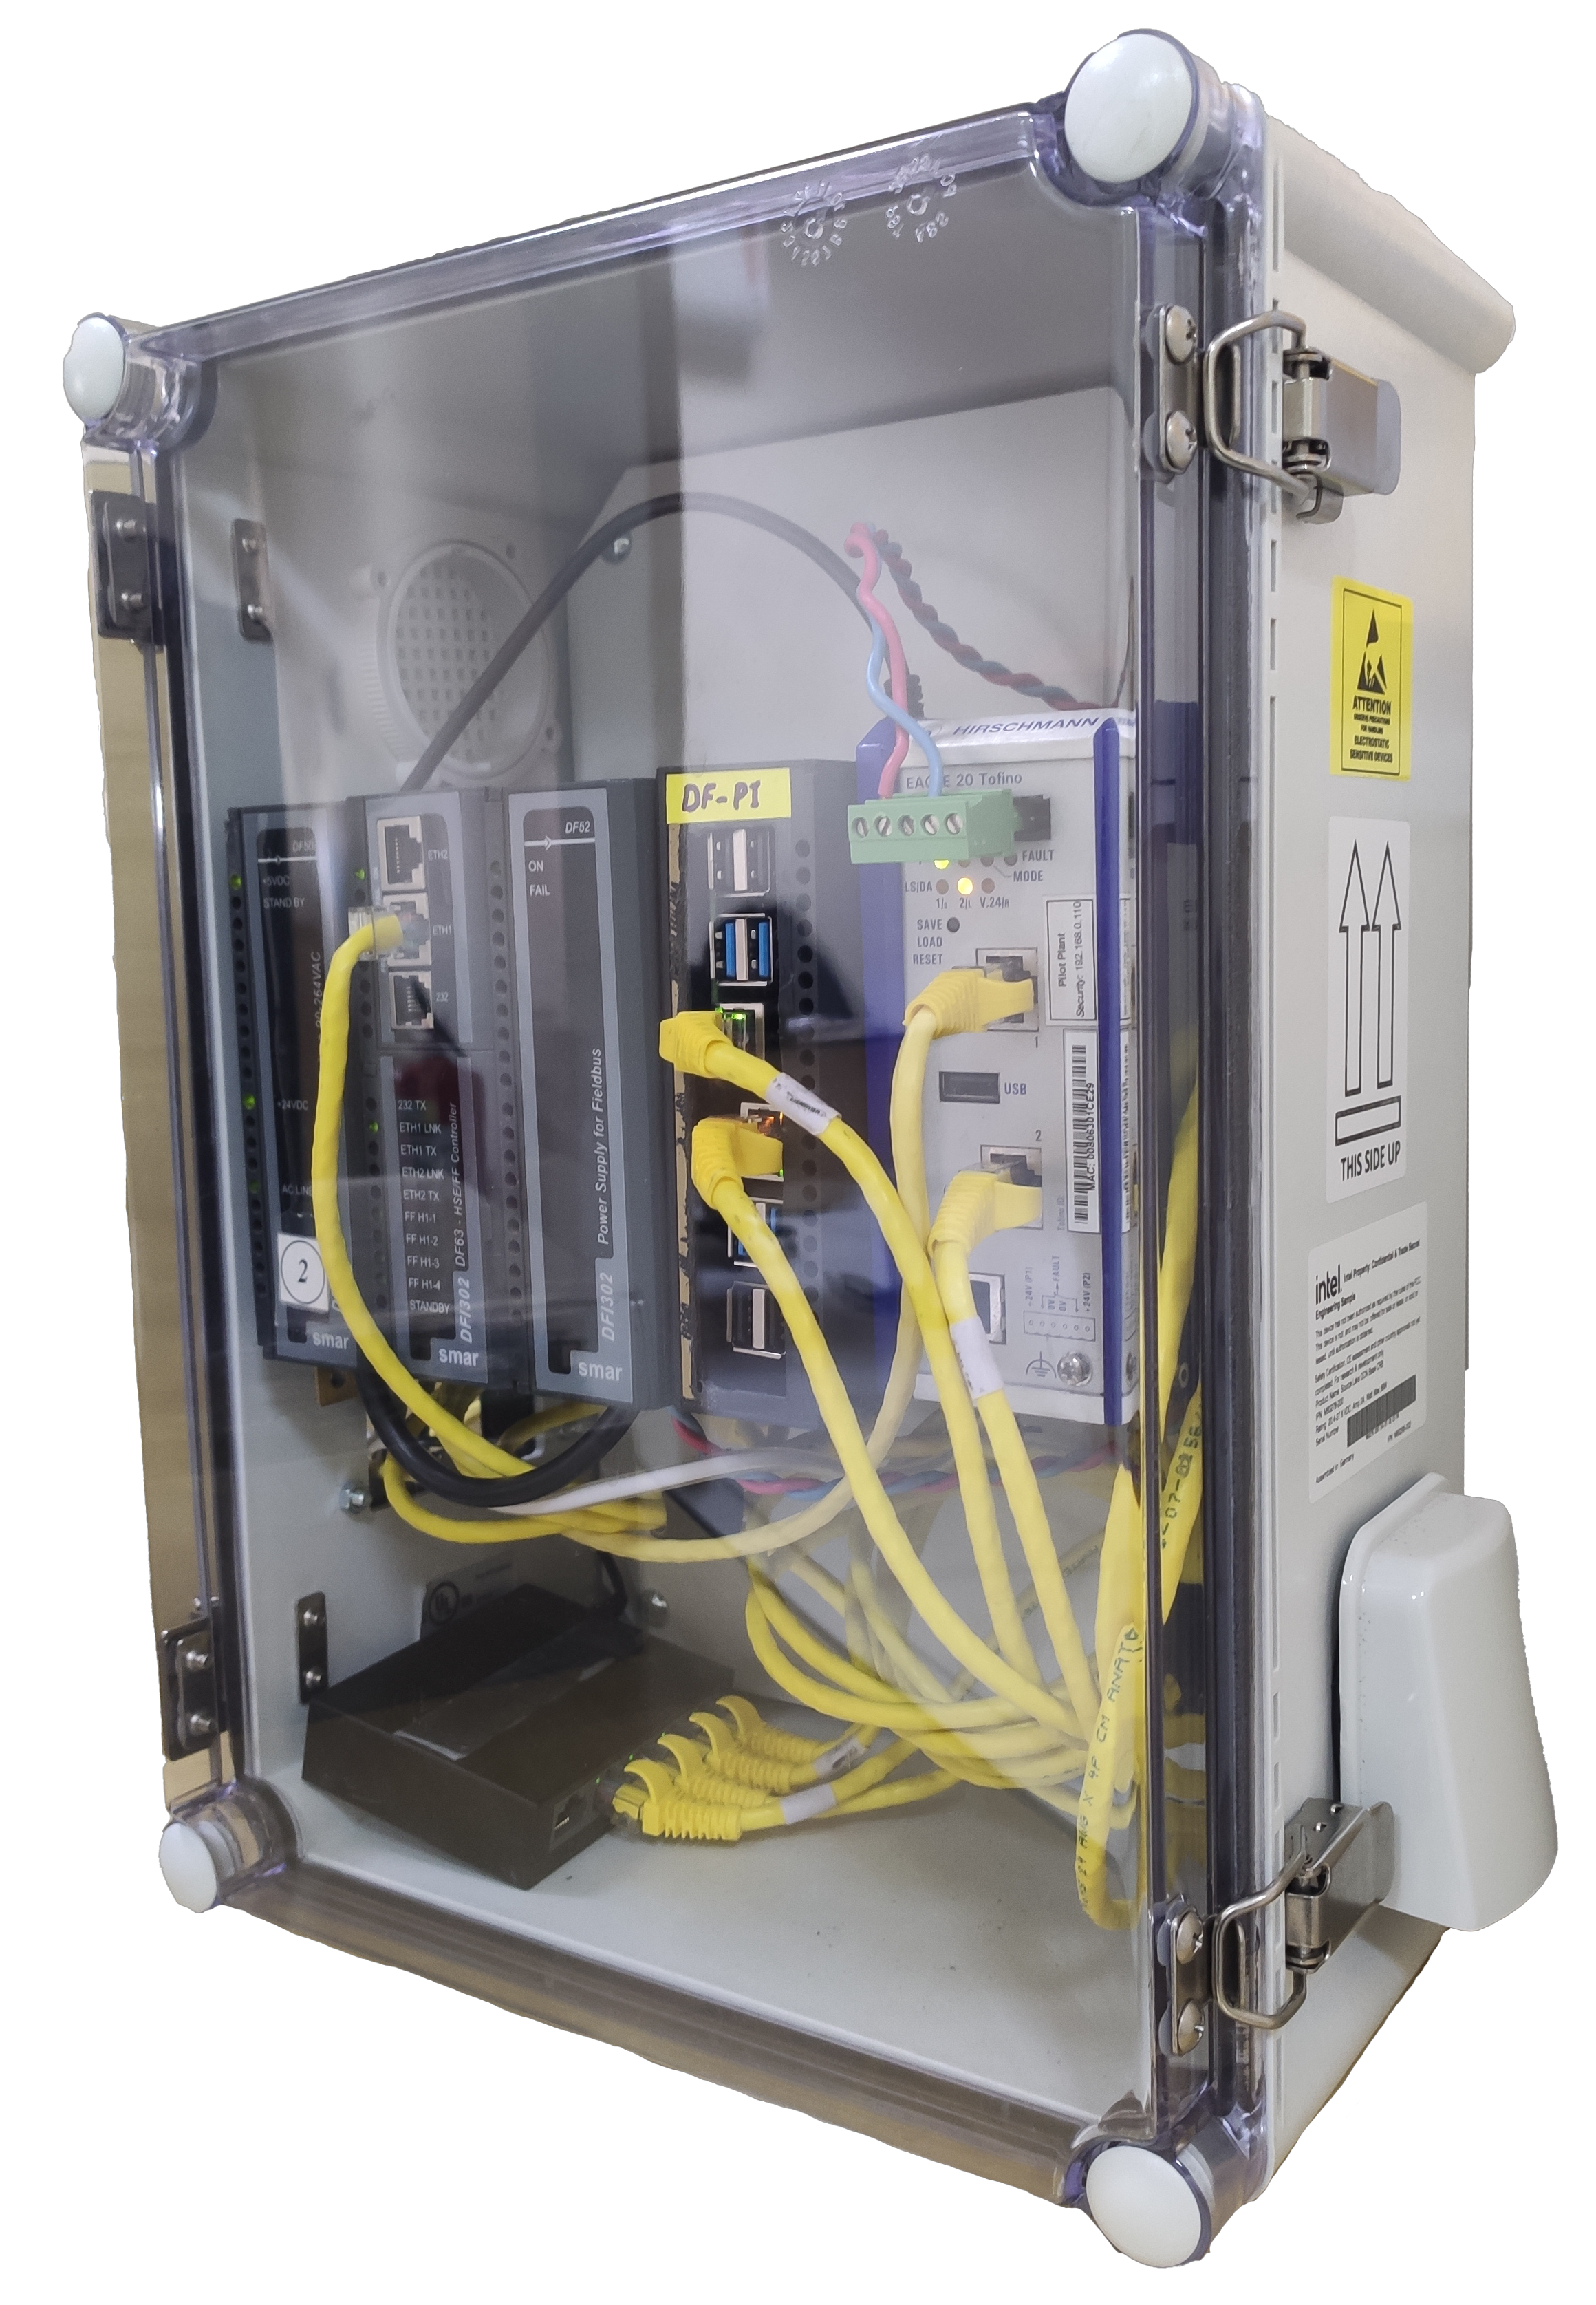
\includegraphics[width=0.5\textwidth]{USPSC-img/cyberkit2.png}
        \end{center}
        \legend{Fonte: elaborada pelo autor.}
    \end{figure}

\section{Aquisição dos Dados nos Cenários de Ataques Cibernéticos} \label{sec:exec-attacks}

No passo da metodologia apresentado pela \autoref{sec:aquisicao}, coloca-se a bancada em operação de acordo com os cenários especificados (\autoref{tab:attacks}), aciona-se o sistema de medição, nas quais são realizadas aquisição do tráfego da rede e do desempenho do hospedeiro do servidor OPC UA, e efetua-se os respectivos ataques. Os dados de processa da rede OPC UA são coletados por 60 segundos para cada cenário.

A \autoref{tab:carac-cenarios} apresenta um resumo detalhado das características do tráfego da rede e desempenho em cada cenário de ataque e comunicação normal em redes OPC UA industriais.

\begin{table}[htbp!]
    \centering
    \caption{Informações do tráfego da rede e desempenho do hospedeiro em cada cenário}%
    \label{tab:carac-cenarios}
    \begin{tabular}{M{1.5cm}M{3cm}M{2.5cm}M{2.5cm}M{2cm}M{2cm}}
        \toprule
        \textbf{Cenário} & \textbf{\textit{Throughput} médio (kbits/s)} & \textbf{TP\textsuperscript{1} médio (Bytes)} & \textbf{PPS\textsuperscript{2} médio (pacotes/s)} & \textbf{Tráfego OPC UA (\%)} & \textbf{CPU\textsuperscript{3} (\%)} \\
        \toprule
        C1 & 130 & 127 & 128.4 & 28.7 & 7.31 \\
        \midrule
        C2 & 175 & 153 & 142.9 & 34.4 & 8.91 \\
        \midrule
        C3 & 179 & 162 & 138.3 & 31.8 & 9.01 \\
        \midrule
        C4 & 1166 & 965 & 151.1 & 9.2 & 17.16 \\
        \midrule
        C5 & 6824 & 972 & 877.9 & 5.3 & 10.64 \\
        \midrule
        C6 & 6894 & 973 & 885.9 & 8.2 & 10.78 \\
        \midrule
        C7 & 18000 & 60 & 38438.9 & 0.1 & 14.68 \\
        \midrule
        C8 & 12000 & 60 & 26788.9 & 0.1 & 13.23 \\
        \midrule
        C9 & 15000 & 60 & 31278.5 & 0.1 & 14.81 \\
        \midrule
        C10 & 462 & 171 & 337.3 & 72.9 & 9.86 \\
        \midrule
        C11 & 501 & 180 & 348.0 & 71.9 & 11.27 \\
        \midrule
        C12 & 491 & 184 & 334.1 & 69.8 & 11.36 \\
        \midrule
        C13 & 196 & 173 & 141.4 & 33.0 & 7.52 \\
        \midrule
        C14 & 235 & 195 & 151.3 & 35.2 & 9.03 \\
        \midrule
        C15 & 247 & 203 & 152.6 & 32.3 & 9.09 \\
        \midrule
        C16 & 105 & 125 & 105.3 & 33.1 & 6.80 \\
        \midrule
        C17 & 146 & 148 & 123.4 & 33.1 & 7.84 \\
        \midrule
        C18 & 137 & 159 & 107.9 & 33.2 & 7.96 \\
        \midrule
        C19 & 3410 & 43 & 10012.0 & 0.2 & 7.36 \\
        \midrule
        C20 & 3433 & 43 & 9896.4 & 0.2 & 7.97 \\
        \midrule
        C21 & 3432 & 44 & 9854.8 & 0.2 & 7.97 \\
        \midrule
        C22 & 168 & 127 & 166.1 & 32.1 & N/A \\
        \midrule
        C23 & 223 & 154 & 182.4 & 34.5 & N/A \\
        \midrule
        C24 & 219 & 162 & 169.7 & 32.5 & N/A \\
        \midrule
        C25 & 95 & 121 & 98.5 & 28.3 & 7.01 \\
        \midrule
        C26 & 253 & 142 & 222.7 & 17.9 & 7.95 \\
        \midrule
        C27 & 234 & 147 & 199.8 & 17.1 & 8.25 \\
        \bottomrule
        \multicolumn{6}{>{\tiny}l}{\textsuperscript{1} Tamanho do pacote.} \\
        \multicolumn{6}{>{\tiny}l}{\textsuperscript{2} Taxa de pacotes por segundo.} \\
        \multicolumn{6}{>{\tiny}l}{\textsuperscript{3} Processamento do hospedeiro do servidor OPC UA.} \\
    \end{tabular}
    \fonte{elaborada pelo autor.}%
\end{table}

O \textit{throughput} médio e a média do tamanho dos pacotes dos cenários variam consideravelmente, indicando a intensidade do tráfego gerado em cada situação. Os diferentes cenários de ataques de DoS pelo loop infinito na cadeia de certificados, como C1, C2 e C3, apresentam uma taxa de transferência de dados relativamente baixa. Em contraste, cenários como C7, C8 e C9, que envolvem DoS pela inundação do TCP/IP, mostram \textit extremamente alto, refletindo a alta carga gerada por esses ataques. Essa carga é demonstrada pelo indicador crítico da intensidade do tráfego, PPS (taxa de pacotes por segundo), que atinge valores elevados nesses cenários.

Já o percentual de tráfego OPC UA, apesar de variar drasticamente entre os cenários, não é considerado isoladamente um fator determinante para a severidade do ataque. Por exemplo, cenários com baixa porcentagem de tráfego OPC UA, como C7, C8 e C9, ainda podem gerar uma carga considerável na rede devido ao alto PPS. Por outro lado, cenários como C10, C11 e C12, que apresentam uma alta porcentagem de tráfego OPC UA, podem não necessariamente implicar em uma alta taxa de pacotes por segundo, mas indicam que o ataque está especificamente direcionado aos protocolos de comunicação OPC UA.

Adicionalmente, o percentual do uso de processamento do controlador industrial (hospedeiro do servidor UA), é um indicador importante da carga imposta ao sistema durante os ataques. Cenários como C4, C5 e C6, que envolvem ataques de DoS pela chamada de vários métodos OPC UA nulos, mostram um aumento significativo no uso da CPU, indicando que esses ataques conseguem sobrecarregar o processamento do controlador, potencialmente levando à degradação do serviço ou à sua interrupção.

Essa análise destaca a importância de considerar múltiplas métricas ao avaliar o impacto dos diferentes tipos de ataques na rede OPC UA. Além da taxa de transferência e de pacotes por segundo, o tamanho dos pacotes e o percentual de tráfego OPC UA são essenciais para uma compreensão abrangente do comportamento da rede sob diferentes condições de ataque. A análise detalhada dessas variáveis pode fornecer insights valiosos para o desenvolvimento de estratégias de mitigação e a implementação de medidas de segurança mais eficazes em ambientes industriais.

\section{Processamento dos Dados} \label{sec:processamento-dados}

Uma vez que os dados de tráfego da rede e desempenho do hospedeiro do servidor OPC UA foram coletados para cada cenário de ataque, o próximo passo é processar esses dados para análise e interpretação. Este processamento é realizado pelo aplicativo \textbf{uanalyser}, que é responsável por extrair informações relevantes dos dados brutos e gerar métricas de desempenho para cada cenário.

Na versão atual do aplicativo (v1.0.0), são gerados gráficos de (a) \textit{Throughput} (kbps), (b) desempenho do hospedeiro do servidor OPC UA (RAM e CPU), (c) quantidade de pacotes OPC UA por segundo e (d) \textit{Round Trip Time} (RTT) normalizado, por pacote. A figura \autoref{fig:0-normal_local_server} apresenta um exemplo dos quatro gráficos de saída do aplicativo para o cenário C25.

\begin{figure}[htbp!]
    \centering
    \begin{subfigure}[t]{0.5\textwidth}
        \centering
        \includegraphics[width=1\textwidth, height=120pt]{USPSC-img/output/cropped/0-normal_local_server-tput.png}
        \caption{\textit{Throughput}}
    \end{subfigure}%
    ~ 
    \begin{subfigure}[t]{0.5\textwidth}
        \centering
        \includegraphics[width=1\textwidth, height=120pt]{USPSC-img/output/cropped/0-normal_local_server-perf.png}
        \caption{Desempenho}
    \end{subfigure}%
    \\
    \begin{subfigure}[t]{0.5\textwidth}
        \centering
        \includegraphics[width=1\textwidth, height=120pt]{USPSC-img/output/cropped/0-normal_local_server-pack.png}
        \caption{Pacotes OPC UA}
    \end{subfigure}%
    ~
    \begin{subfigure}[t]{0.5\textwidth}
        \centering
        \includegraphics[width=1\textwidth, height=120pt]{USPSC-img/output/cropped/0-normal_local_server-rttp.png}
        \caption{RTT por pacote}
    \end{subfigure}%
    \label{fig:0-normal_local_server}
    \caption{Gráficos de condição normal de operação - nível de segurança: `None'.}
\end{figure}

Os demais gráficos gerados para os outros cenários podem ser visualizados no \autoref{ap:graficos}.

\section{Análise dos Resultados} \label{sec:analise-resultados}

Nesta seção, são apresentadas as análises dos resultados obtidos a partir dos cenários de ataques cibernéticos executados na bancada experimental. A análise é realizada com base nas métricas de desempenho extraídas dos dados brutos coletados, com o objetivo de avaliar a robustez das redes industriais OPC UA e a variação no desempenho dos componentes ao serem submetidos a tais cenários. Com isso, para organizar melhor as informações, os resultados são divididos em seções que correspondem a cada tipo de ataque

\subsection{\textit{Packet Sniffing}}

Com o auxílio do Wireshar e do Ettercap, este primeiro ataque foi proferido com o objetivo de identificar a presença de vulnerabilidades na rede OPC UA que permitam a interceptação não autorizada de pacotes. Inicialmente, o Ettercap foi empregado para a captura unificada de pacotes, enquanto o Wireshark foi utilizado para a análise detalhada do tráfego de rede. Uma vez que o servidor e o cliente estão conectados, um canal seguro para comunicação é estabelecido. No entanto, o atacante pode explorar vulnerabilidades na rede para interceptar pacotes e obter informações confidenciais, como endereços IP e MAC de todos os dispositivos conectados. No início da captura para o cenário C22, C23 e C24, é possível observar a presença de pacotes de comunicação entre o servidor e o cliente, conforme ilustrado na \autoref{fig:packet-sniffing}.

\subsection{\textit{Man in the Middle (MITM)}}

\subsection{\textit{Denial of Service (DoS)}}

\section{Propostas de Melhorias e Mitigações} \label{sec:melhorias-mitigacoes}

\subsection{Recomendações para Comunicações Seguras com o Protocolo OPC UA}

Como resultado de uma série de testes realizados em conformidade com os padrões de segurança, foram identificadas e resumidas as seguintes recomendações para o uso de comunicações seguras com o protocolo OPC UA:

\begin{itemize}
    \item \textbf{Operação no "SecurityMode"}: É essencial selecionar os modos `Sign' ou `Sign \& Encrypt'. Esses modos garantem que, no nível da aplicação, a autenticação seja obrigatória. O modo de segurança `None' não oferece proteção alguma! O modo de segurança `Sign \& Encrypt' é utilizado para proteger a integridade dos dados e sua confidencialidade.
    \item \textbf{Escolha dos Algoritmos Criptográficos}: Deve-se selecionar `Basic256Sha256' como a \textit{Security Policy}, desde que os clientes com os quais o servidor interage suportem essa política. Políticas de segurança que utilizam algoritmos obsoletos, como `SHA-1', não devem ser utilizadas.
    \item \textbf{Autenticação de Usuários}: O login no servidor UA com um ID `anônimo' deve ser utilizado apenas ao acessar recursos não críticos, pois, nesse caso, não é possível rastrear quem está alterando os dados ou a configuração. Hackers podem explorar essas recomendações para usar o OPC UA com um ID seguro para ler ou escrever dados de maneira não autorizada. Isso pode ocorrer se a restrição dos direitos de trabalho com o identificador `anônimo' não for configurada adequadamente.
    \item \textbf{Armazenamento de Certificados e Chaves Privadas}: As chaves privadas ou arquivos de certificado utilizados não devem ser armazenados em um sistema de arquivos não criptografado. Para esse propósito, devem ser usados armazenamentos especiais de certificados do sistema operacional e suas capacidades para definir direitos de acesso. Recomenda-se o uso de TPMs (\textit{Trusted Platform Modules}) ou hardware seguro externo, como tokens de autenticação USB, para armazenar certificados e/ou chaves privadas.
    \item \textbf{Uso de Certificados}: Conexões que não fornecem certificados confiáveis não são permitidas. Certificados autoassinados requerem verificação adicional. Se os certificados não forem autoassinados, é necessário o estabelecimento de uma autoridade certificadora, e os certificados dessa autoridade devem ser assinados de forma independente ou por outra autoridade certificadora. As autoridades certificadoras podem ser multinível.
    \item \textbf{Gestão e Manutenção de Certificados}: Recomenda-se o uso de listas de confiança de certificados e listas de revogação de certificados para gerenciar apenas certificados válidos. Essas listas são criadas por usuários ou processos confiáveis e devem ser atualizadas regularmente.
\end{itemize}

% \section{Resultados Esperados}

% Na busca por aprimorar a cibersegurança dos sistemas de controle e automação industrial por meio de uma análise meticulosa das vulnerabilidades em redes OPC UA, é imperativo delinear os resultados esperados da metodologia aplicada no presente trabalho. As expectativas de resultados estão fundamentadas em uma avaliação abrangente da robustez da rede e variações no desempenho dos controladores ao serem submetidos aos cenários de ataque cibernético apresentados na \autoref{sec:attacks}.

% Primeiramente, no que se refere à simulação de ataques de \textit{Packet Sniffing}, espera-se que as redes OPC UA demonstrem um alto nível de resistência à interceptação não autorizada de pacotes, decorrente do modo de segurança inerente ao protocolo utilizado. O maior nível de proteção é apresentado pelo modo \textbf{Sign\&Encrypt}, no qual inclui recursos de criptografia e autenticação. Consequentemente, as informações trocadas entre cliente e servidor OPC UA permanecem confidenciais, íntegras e disponíveis (CIA), garantindo assim a segurança da rede.

% Em segundo lugar, no contexto de ataques do tipo \textit{Man-in-the-Middle} (MITM), é imperativo considerar a detecção e prevenção destas intrusões, também com uma dependência significativa do modo de segurança selecionado. Semelhante ao cenário de ataque anterior, uma configuração que priorize o mais alto nível de segurança e a seleção adequada de políticas de criptografia devem, a princípio, proteger a rede OPC UA contra ataques MITM perpetrados por um possível Elemento Invasor. Entretanto, em situações que existam vulnerabilidades conhecidas na rede e em sua configuração, como a utilização do modo \textbf{None}, um elemento não confiável pode explorar tais fragilidades para corromper a tabela ARP (\textit{ARP Spoofing}), permitindo a interceptação das informações transmitidas entre o cliente e o servidor. Além disso, esse invasor pode modificar potencialmente dados por meio da inserção de algum \textit{malware}.

% Por fim, no que diz respeito a ataques de negação de serviço (DoS), é importante considerar que os resultados esperados podem diferir dos observados nos ataques mencionados anteriormente, dependendo da capacidade da rede e de processamentos dos componentes \textit{hosts} do servidor OPC UA. Antecipa-se que, embora o ambiente experimental desenvolvido compreenda apenas alguns dispositivos de redes e não incorpore preocupações com a capacidade de comunicação, a correta avaliação dos dados capturados nos cenários simulados deverá evidenciar que esse ataque pode prejudicar a troca de mensagens ao esgotar os recursos de uma rede com grande composição. Estima-se, ainda, que os danos sejam mais significativos quando se utiliza o modo de segurança \textbf{Sign\&Encrypt} e quando o inunda com os pacotes referentes a validações de certificado e ao processo de criptografia.

% Além disso, a pesquisa se esforça para fornecer informações valiosas sobre vulnerabilidades potenciais que podem ser expostas durante o processo de experimentação. Estas prospecções, caso confirmadas, auxiliam em avanços futuros do protocolo OPC UA e de sistemas IACSs, fortalecendo ainda mais a robustez destes e resistência contra ameaças cibernéticas em constante evolução.
